\documentclass[10pt]{article}
\usepackage{titlesec}
\usepackage{geometry}
\geometry{verbose,tmargin=.9in,bmargin=.9in,lmargin=1.0in,rmargin=1.0in}
\usepackage{amsmath,amsfonts,amsthm,amssymb}
\usepackage{url}
\usepackage{color}
\usepackage[usenames,dvipsnames,svgnames,table]{xcolor}
\usepackage[colorlinks=true, linkcolor=red, urlcolor=blue, citecolor=gray]{hyperref}
\usepackage{float}
\usepackage{caption}
\usepackage{subcaption}
\usepackage{graphicx}
\usepackage{wrapfig}
\usepackage{booktabs}
\usepackage{longtable}
\usepackage{enumitem}
\usepackage{multicol}
\usepackage{etoolbox}

\definecolor{nyuDarkPurple}{HTML}{330662}
\definecolor{nyuOfficialPurple}{HTML}{57068c}

\newcommand{\spara}[1]{\vspace{.5em}\noindent {\large\sffamily\textcolor{nyuOfficialPurple}{#1}}}
\titleformat{\section}[hang]{\Large\sffamily\color{nyuDarkPurple}}{\thesection}{1em}{}
\titleformat{\subsection}[hang]{\large\sffamily\color{nyuDarkPurple}}{\thesection}{1em}{}
\titleformat{\subsubsection}[hang]{\normalsize\sffamily\color{gray}}{\thesection}{1em}{}

\usepackage{fancyhdr}
\pagestyle{fancy}
\lhead{
\includegraphics[width=4cm]{tandon_long_color.eps}}
\rhead{\thepage}
\pagenumbering{gobble}

\setcounter{secnumdepth}{0}

% math commands
\DeclareMathOperator{\R}{\mathbb{R}}
\newcommand{\E}{\mathbb{E}}
\DeclareMathOperator{\Var}{Var}
\newcommand{\bs}[1]{\boldsymbol{#1}}
\newcommand{\bv}[1]{\mathbf{#1}}

\usepackage{bbm}

\begin{document}
	
\begin{center}
	\normalsize
	New York University Tandon School of Engineering
	
	Computer Science and Engineering
	\medskip
	
	\large
	CS-GY 6763: Homework 2. 
	
	Due Thursday, February 20th, 2025, 11:59pm ET.
	\medskip
	
	\normalsize 
	\noindent \emph{Collaboration is allowed on this problem set, but solutions must be written-up individually. Please list collaborators for each problem separately, or write ``No Collaborators" if you worked alone.}

\end{center} 

\subsection{Problem 1: Exploring Concentration Bounds}
\textbf{(8 pts)} Let $X$ be a random variable uniformly distributed in the interval $[0,1]$. Since we know $X$'s distribution exacty, we can easily check that $\Pr[X \geq 7/8] = 1/8$. But let's take a look at what various concentration inequalities would predict about this probability using less information about $X$. 
\begin{enumerate}
	\item Given an upper bound on $\Pr[X \geq 7/8]$ using Markov's inequality. 
	\item Give an upper bound on $\Pr[X \geq 7/8]$ using Chebyshev's inequality.
	\item Given an upper bound on $\Pr[X \geq 7/8]$ by applying Markov's inequality to the random variables $X^2$ (the ``raw'' second moment). 
	Note that this is slightly different than using Chebyshev's inequality, which applies Markov to the ``central'' second moment $(X - \E[X])^2$.
	\item What happens for higher moments? Applying Markov's to $X^q$ for $q = 3,4, \ldots, 10$. Describe what you see in a sentence. What value of $q$ gives the tightest bound?
		\item One take-away here is that, depending on the random variable being studied, it is not always optimal to use the variance as a deviation measure to show concentration. Markov's can be used with any monotonic function $g$, and as we see above, different choices might give better bounds. Exhibit a monotonic function $g$ so that applying Markov’s to $g(X)$ gives as tight an upper bound on $\Pr[X \geq 7/8]$ as you can. Maximum points if you can get $\Pr[X \geq 7/8] \leq 1/8$, which would be the best possible.
\end{enumerate}
% f does not need to be strictly monotonic! Why? Sort of counterintuitive but got a question about this last year. 


\subsection{Problem 2: Boosting Success Probability}
\textbf{(12 pts)}
We saw in class that computing the \emph{mean} of many different answers from a randomized algorithm is often an effective way to improve accuracy. It turns out that the \emph{median} is also very useful: it can be used to improve \emph{success probability}. 

In particular, suppose our goal is to estimate some scalar quantity $f(X)$ of a dataset $X$ (e.g, the number of distinct items in a stream). Suppose we have developed a high-accuracy randomized algorithm, $\mathcal{A}$, but it only succeeds with probability $\geq 2/3$. I.e., on any input $X$, with with probability $\geq 2/3$,
\begin{align*}
	|\mathcal{A}[X] - f(X)| \leq \epsilon
\end{align*}

Prove that, if we run $\mathcal{A}$ a total of $r = O(\log(1/\delta)$ times with different random seeds and return the \emph{median}, $M$, of the $r$ outputs, then with probability $1-\delta$:
\begin{align*}
		|M - f(X)| \leq \epsilon.
\end{align*}
This approach could be used, for example, to obtain an $O(\log(1/\delta)/\epsilon^2)$ space algorithm for distinct items, whereas in class we only proved $O(1/\delta\epsilon^2)$ using Chebyshev's inequality. 

\vspace{1em}
\noindent \textbf{Hint:} Think about what event would have to happen for the median to be ``bad'', i.e., to give error $> \epsilon$. If the median is bad, what does it say about the fraction of our $r$ estimates that are bad?



% \subsection{Problem 4: Exploring Concentration Bounds. (8 pts)}
% Using combinatorics, write down and evaluate (e.g., run some code) an exact expression for the probability of flipping 60 or more heads when flipping a fair coin 100 times. Do the same for 600 or more heads in 1000 flips. Compare your results to the upper bound given by the Chernoff bound from Lecture 2:
% \begin{align*}
% 	\Pr[S > (1+\epsilon)\mu] \leq e^{-\frac{\epsilon^2\mu}{2+\epsilon}}.
% \end{align*}
% Also compare to this slightly different and less commonly used form of the bound from Wikipedia:
% \begin{align*}
% 	\Pr[S > (1+\epsilon)\mu] \leq \left(\frac{e^\epsilon}{(1+\epsilon)^{1+\epsilon}}\right)^{\mu}.
% \end{align*}
% Also compute what each Chernoff Bound would give if you wanted to bound the probability of flipping more than 70 or 700 heads. 
% Write a 1-2 sentence comment on how what your findings suggest about how ``tight'' the Chernoff bound is. 

\subsection{Problem 3: Hashing around the clock.}

\textbf{(15 pts)} In modern systems, hashing is often used to distribute data items or computational tasks to a collection of servers. What happens when a server is added or removed from a system? Most hash functions, including those discussed in class, are tailored to the number of servers, $n$, and would change completely if $n$ changes. This would require rehashing and moving all of our $m$ data items, an expensive operation.

\begin{figure}[h]
	\centering
	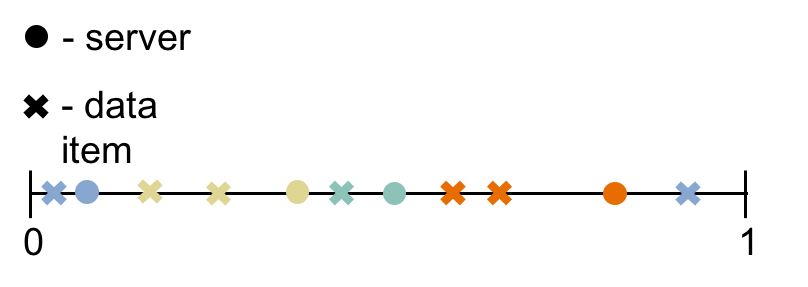
\includegraphics[width=0.7\textwidth]{consistentHashing.png}
	\caption{Each data item is stored on the server with matching color.}
\end{figure}


Here we consider an approach to avoid this problem. Assume we have access to a completely random hash function that maps any value $x$ to a real value $h(x) \in [0,1]$. Use the hash function to map \emph{both} data items and servers randomly to $[0,1]$. Each data item is stored on the first server to its right on the number line (with wrap around -- i.e. a job hashed below 1 but above all serves is assigned to the first server after 0). When a new server is added to the system, we hash it to $[0,1]$ and move data items accordingly.

\begin{enumerate}
	\item Suppose we have $n$ servers initially. When a new server is added to the system, what is the expected number of data items that need to be relocated? 
	
	\item Show that, with probability $>9/10$, no server ``owns'' more than an $O(\log n /n)$ fraction of the interval $[0,1]$. 
	\textbf{Hint:} This can be proven \underline{without} a concentration bound.
	
	\item Show that if we have $n$ servers and $m$ items and $m > n$, the maximum load on any server is no more than $O(\frac{m}{n}\log n)$ with probability $> 9/10$. 
\end{enumerate}

%\subsection{Problem 1: Johnson-Lindenstrauss Approximates Inner Products.}
%\textbf{(10 pts)}
%\begin{enumerate}
%\item Suppose that $\Pi$ is a Johnson-Lindenstrauss matrix with $k = O\left(\frac{\log(1/\delta)}{\epsilon^2}\right)$ rows. Prove that for any $x, y$:
%\begin{align*}
%	|\langle x,y\rangle - \langle \Pi x,\Pi y\rangle| \leq \epsilon (\|x\|_2^2 + \|y\|_2^2)
%\end{align*}
%with probability $\geq 1-\delta$. \textbf{Hint:} Try exploiting connections between norms and inner products.
%\item Show that a better bound can be obtained by augmenting our sketches with the norms of each vector. I.e., instead of just $\Pi x$ and $\Pi y$, store as the sketches for $x$ and $y$ both $(\Pi x, \|x\|_2)$ and $(\Pi y, \|y\|_2)$ and show that using these sketches we can compute an estimate $z$ such that 
%\begin{align*}
%	|\langle x,y\rangle - z| \leq \epsilon (\|x\|_2\|y\|_2)
%\end{align*}
%with $1-\delta$ probability when  $k = O\left(\frac{\log(1/\delta)}{\epsilon^2}\right)$. By the AM-GM inequality, we always have that $\|x\|_2\|y\|_2 \leq \|x\|_2^2 + \|y\|_2^2$.
%\end{enumerate}

\subsection{Problem 4(a): Analyzing Sign-JL and JL for Inner Products }
\textbf{(15 pts)}
Often practitioners prefer JL matrices with discrete random entries instead of Gaussians because they take less space to store and are easier to generate. We  analyze one construction below.

Suppose that $\bs{\Pi}$ is a ``sign Johnson-Lindenstrauss matrix'' with $n$ columns, $k$ rows, and i.i.d. $\pm 1$ entries scaled by $1/\sqrt{k}$. In other words, each entry in the matrix has values $-1/\sqrt{k}$ with probability $1/2$ and $1/\sqrt{k}$ with probability $1/2$.
\begin{enumerate}
	\item Prove that for any vector $\bv{x}\in \R^n$, $\E[\|\bs{\Pi}\bv{x}\|_2^2] = \|\bv{x}\|_2^2$ and that $\Var[\|\bs{\Pi}\bv{x}\|_2^2] \leq \frac{2}{k}\|\bv{x}\|_2^4$. This is the meat of the problem and will take some effort. 
	\vspace{.5em}

%	\textit{Observe that if you work through the analysis in class, a random Gaussian JL matrix leads to variance $\frac{2}{k}\|\bv{x}\|_2^4$, so the sign-JL matrix yields strictly lower variance estimator.}
	
	\item Use the above to prove that $\Pr\left[\left|\|\bs{\Pi}\bv{x}\|_2^2 - \|\bv{x}\|_2^2\right| \geq \epsilon\|\bv{x}\|_2^2 \right] \leq \delta$ as long as we choose $k = O\left(\frac{1/\delta}{\epsilon^2}\right)$. Note that this bound almost matches the distributed JL lemma proven in class, but with a worse failure probability dependence of $1/\delta$ in place of $\log(1/\delta)$. 
	\vspace{.5em}
	
	\textit{With more work, it's possible to improve the dependence to $\log(1/\delta)$ for the sign-JL matrix, but we won't do so here.}
	
	\item Generalize your analysis above to show that JL matrices are also useful in approximating inner products between two vectors. For vectors $\bv{x},\bv{y}\in \R^n$ prove that $\Pr\left[\left|\langle \bs{\Pi}\bv{x}, \bs{\Pi}\bv{y}\rangle -  \langle  \bv{x}, \bv{y}\rangle\right| \geq \epsilon\|\bv{x}\|_2\|\bv{y}\|_2\right] \leq \delta$ as long as we choose $k = O\left(\frac{1/\delta}{\epsilon^2}\right)$.
	
		\textit{This result can also be improved to have a $\log(1/\delta)$ dependence in place of $1/\delta$. .}
\end{enumerate}

\subsection{Problem 4(b): Join Size Estimation}
\noindent\textbf{(5 pts)}
One powerful application of sketching is in database applications. For example, a common goal is to estimate the \emph{inner join size} of two tables without performing an actual inner join (which is expensive, as it requires enumerating the keys of the tables). Formally, consider two sets of unique keys $X = \{x_1, \ldots, x_m\}$ and $Y = \{y_1, \ldots, y_n\}$ which are subsets of $1,2, \ldots, U$.  Our goal is to estimate $|X\cap Y|$ based on small space compressions of $X$ and $Y$.  

Using your result from Problem 1, describe a method based on inner product estimation that constructs independent sketches of $X$ and $Y$ of size  $k = O\left(\frac{1}{\epsilon^2}\right)$ and from these sketches can return an estimate $Z$ for $|X\cap Y|$ satisfying
\begin{align*}
	\left|Z - |X\cap Y|\right| \leq \epsilon \sqrt{|X||Y|}
\end{align*}
with probability $9/10$.

%\subsection{Problem 3: If at first you don't success, try again.}
%\textbf{(10 pts)} In class, we saw that, when hashing $m$ items into a hash table of size $O(m^2)$, the expected number of collisions was $< 1$. In particular, this meant we could easily find a ``perfect'' hash function of the table that has no collisions.
%
%Consider the following alternative scheme: build two tables, each of size $O(m^{1.5})$ and choose a separate random hash function for each table. To insert an item, hash it to one bucket in each table and place it in the emptier bucket.
%
%\begin{enumerate}
%	\item Show that, if we're hashing $m$ items, with probability $1/2$, there will be no collisions in either table. You may assume a \underline{fully random hash function}.
%	\item Modify the above scheme to use $O(\log m)$ tables. Prove that this approach yields a collision-free hashing scheme with space $O(m  \log m)$. Again, you may assume a fully random hash function.
%\end{enumerate}


% \subsection{Problem 3: Compressed classification.}
% \textbf{(10 pts)} In machine learning, the goal of many classification methods (like support vector machines) is to separate data into classes using a \emph{separating hyperplane}.

% Recall that a hyperplane in $\R^d$ is defined by a unit vector $a \in \R^d$ ($\|a\|_2 = 1$) and scalar $c \in \R$. It contains all  $h \in \R^d$ such that $\langle a, h\rangle = c$. 

% Suppose our dataset consists of $n$ unit vectors in $\R^d$ (i.e., each data point is normalized to have norm $1$). These points can be separated into two sets $X, Y$,
% with the guarantee that there exists a hyperplane such that every point in $X$ is on one side and every point in 
% $Y$ is on the other. In other words, for all $x\in X, \langle a, x\rangle > c$ and for all $y\in Y, \langle a, y\rangle < c$.

% Furthermore, suppose that the $\ell_2$ distance of each point in $X$ and $Y$ to this separating hyperplane is at least $\epsilon$. When this is the case, the hyperplane is said to have ``margin'' $\epsilon$. 

% \begin{enumerate}
% 	\item Show that this margin assumption equivalently implies that for all $x\in X, \langle a, x\rangle \geq c + \epsilon$ and for all $y\in Y, \langle a, y\rangle \leq c - \epsilon$.
	
% 	\item Show that if we use a Johnson-Lindenstrauss map $\Pi$ to reduce our data points to $O(\log n/\epsilon^2)$ dimensions, then the dimension reduced data can still be separated by a hyperplane with margin $\epsilon/4$, with high probability (say $> 9/10$).
% \end{enumerate}

% \subsection{Problem 4: LSH in the Wild} 
% \textit{This exercise does not involve formal proofs or analysis like more typical problem set problems. It will likely involve some coding or spreadsheet work.}
% \vspace{.25em}

% \noindent\textbf{(10 pts)}
% To support its largely visual platform, Pinterest runs a massive image de-duplication operation built on Locality Sensitive Hashing for Cosine Similarity. You can read about the actual system \href{https://medium.com/pinterest-engineering/detecting-image-similarity-using-spark-lsh-and-tensorflow-618636afc939}{here}. All information and numbers below are otherwise purely hypothetical.

% Pinterest has a database of $N = $ \textbf{1 billion} images. Each image in the database is pre-processed and represented as a vector $\bv{q}\in \R^d$. When a new image is pinned, it is also processed to form a vector $\bv{y} \in \R^d$. The goal is to check for any existing duplicates or near-duplicates to $\bv{y}$ in the database.  
% Specifically, Pinterest would like to flag an image $\bv{q}$ as a near-duplicate to $\bv{y}$ if $\cos(\theta(\bv{q},\bv{y})) \geq .98$. We want to find any near-duplicate with probability $\geq 99\%$. 

% Given this requirement, your job is to design a multi-table LSH scheme using SimHash to find candidate near-duplicates, which can then be checked directly against $\bv{y}$. To support this task, Pinterest has collected data on the empirical distribution of $\cos(\theta(\bv{q},\bv{y}))$ for a typical new image $\bv{y}$. It roughly follows a bell-curve:

% \begin{figure}[H]
% 	\centering
% 	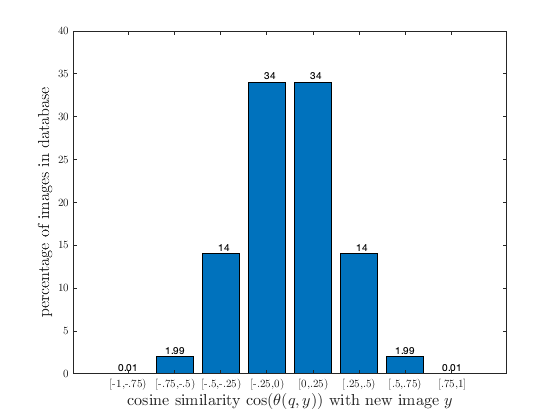
\includegraphics[width=.6\textwidth]{dist.png}
% \end{figure} 

% Pinterest wants to consider two possible computational targets for your LSH scheme, which will determine the speed of the de-duplication algorithm:
% \begin{enumerate}
% 	\item Ensure that no more than $1$ million candidate near-duplicates are checked on average when a new image is pinned. ``Checked'' means that the image's cosine similarity with the new image is computed explicitly, which is a computationally expensive operation.
% 	\item Ensure that no more than $200,000$ candidates are checked on average when a new image is pinned.
% \end{enumerate}

% \noindent Based on the data above, describe how to set parameters for your LSH scheme to minimize the space (i.e., number of tables) used, while achieving each of the above goals. Justify your answers, and any assumptions you make.
% If you code anything up to help calculate your answer, please attach the code. As in lecture, you can assume that each hash table has $m = O(N)$ slots and this is large enough to ignore lower order terms depending on $1/m$. 


\end{document}